\section{Tabular Data Generation with Probabilistic Circuits}


\begin{frame}[fragile]{The Problem}

    \textbf{Q3}: Can we train tractable yet expressive generative models for tabular data?
    \bigskip

    \textbf{The Context}:
    \begin{itemize}
        \item The landscape of tabular data generation is currently dominated by deep generative models.
        \item Unconditional sampling is often the only exact probabilistic query they can compute.
        \item The state of the art is represented by diffusion models, which often show "saturated" performance on standard benchmarks.
    \end{itemize}

    \textbf{Idea}: Use probabilistic circuits, which are tractable models, as tabular data generators.

    % \textbf{Research Questions}:
    % \begin{itemize}
    %     \item Q1: Can we train tractable yet expressive generative models for tabular data?
    %     \item Q2: Do the saturated metrics on standard benchmarks reflect the true quality of the generated data?
    % \end{itemize}

    
\end{frame}

% \begin{frame}[fragile]{Contribution}

%     % \textbf{Q3}: Can we train tractable yet expressive generative models for tabular data?

%     % \textbf{Contribution:}
%     \begin{enumerate}
%         \item We propose an adaptation of probabilistic circuits for tabular data generation, which are tractable models.
%         \item We evaluate the quality of the generated data on common benchmarks of metrics and baselines recently used by state-of-the-art diffusion-based methods.
%         \item We analyze the limitations of current metrics and benchmarks and propose improvements. 
%     \end{enumerate}
    
% \end{frame}

\begin{frame}[fragile]{Probabilistic Circuits (Hierarchical Mixture Models)}

    \begin{columns}
        \column{0.6\textwidth}

    Probabilistic circuits (PC) are tractable models where the density function $p(\mathbf{x})$ is defined as a computational graph composed of three types of nodes:
    \begin{itemize}
        \item \textbf{Input nodes}: tractable distributions $q_\theta(x)$ (ex: $\mathcal{N}(x \mid \mu, \sigma^2)$)

        \item \textbf{Sum nodes}: mixture of distributions (defined over the same variables) $p(\mathbf{x}) = \sum_{i} w_i q_i(\mathbf{x})$
        
        \item \textbf{Product nodes}: product of distributions (defined over different variables) $p(\mathbf{x}) = \prod_{i} q_i(x_i)$
        
    \end{itemize}
    \smallskip
    Model parameters $w_i$ and $\theta$ are learnable by maximum likelihood and gradient-based optimization.

    \smallskip
    The structure is a hyperparameter, usually built with heuristics.

        \column{0.4\textwidth}
            \begin{figure}
                \centering
                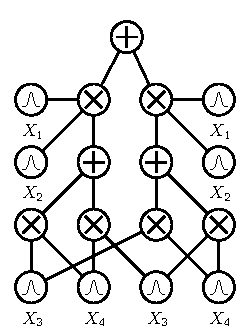
\includegraphics[width=0.95\textwidth]{assets/images/pc_example.pdf}
            \end{figure}
    \end{columns}
    
\end{frame}



% \begin{frame}[fragile]{Probabilistic Circuits}

%     \begin{columns}
%         \column{0.6\textwidth}

%     Probabilistic circuits (PC), are probabilistic models where the density function $p(\mathbf{x})$ is represented as a computational graph composed of three different types of nodes:
%     \begin{itemize}
%         \item \textbf{Input nodes}: $f_\theta(x)$

%         \item \textbf{Sum nodes}: $p(\mathbf{x}) = \sum_{i} w_i p_i(\mathbf{x})$
        
%         \item \textbf{Product nodes}: $p(\mathbf{x}) = \prod_{i} p_i(\mathbf{x})$
        
%     \end{itemize}
    
%     The model parameters are $w_i$  and $\theta$.
    
%     The structure is a hyperparameter.

%         \column{0.4\textwidth}
%             \begin{figure}
%                 \centering
%                 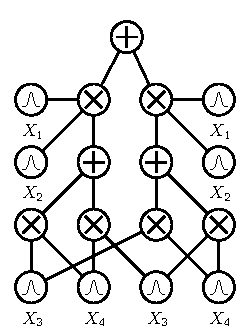
\includegraphics[width=0.95\textwidth]{assets/images/pc_example.pdf}
%             \end{figure}
%     \end{columns}
    
% \end{frame}



% \begin{frame}[fragile]{Structure and Tractability}

%     \begin{columns}
%         \column{0.6\textwidth}
%            Tractability is guaranteed when satisfying the following \textbf{structural constraints}:
    

%        \begin{itemize}

%             \item Multiply functions defined on disjoint sets of variables. Ex: $p(x_1, x_2) = a(x_1) b(x_2)$

%             \item Sum functions defined over identical sets of variables. Ex: $p(x_1, x_2) = w_1 a(x_1,x_2) + w_2 b(x_1, x_2)$

%         \end{itemize}

%         Moreover, if
%         \begin{itemize}
%             \item Input units are tractable probability distributions (e.g., Gaussians, Categorical, etc.)
%             \item Weights of sum nodes are $\geq 0$ and sum to one
%         \end{itemize}

%         The circuit represents a tractable probability distribution.
        
%         \column{0.4\textwidth}
%             \begin{figure}
%                 \centering
%                 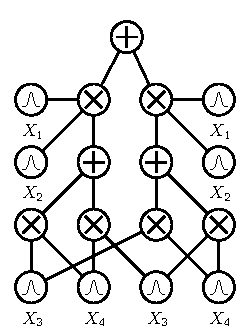
\includegraphics[width=0.95\textwidth]{assets/images/pc_example.pdf}
%             \end{figure}
%     \end{columns}

% \end{frame}


\begin{frame}[fragile]{Tractable Queries}

    Probabilistic circuits allow the following inference queries to be computed in time linear in the size of the circuit:
    \begin{itemize}
        \item \textbf{Density Evaluation} by bottom-up evaluation of the circuit

        \item \textbf{Sampling} by latent ancestral sampling
        
        \item \textbf{Marginalization} of any subset of variables. This is done by setting input units of marginalized variables to 1.
        
        \item \textbf{Conditional Sampling} conditioned on any subset of variables
    \end{itemize}

\end{frame}


% \begin{frame}[fragile]{Learning}

%     A probabilistic circuit is defined by its structure and parameters. 
    
%     \begin{itemize}
%         \item Parameters are the weights of the sum nodes and the parameters of the input distributions. They can be learned by Maximum Likelihood Estimation (MLE) with gradient-based optimization.
%         \item Learning the structure of the circuit is a more complex problem. Often it is fixed with heuristics based on the data.
%         \item Input units are also often fixed to simple distributions.
%     \end{itemize}
    
% \end{frame}

% \begin{frame}[fragile]{Increasing the Expressiveness of Probabilistic Circuits}

%     In order to build generative models for tabular data, we need to increase the expressiveness of probabilistic circuits. We can do this by exploiting recently developed techniques for PCs, such as:
    
%     \begin{itemize}
%         \item \textbf{Overparameterization}: Use a large number of parameters to increase the expressiveness of the model.
        
%         % \item \textbf{Heterogeneous Input Distributions}: Adapt the input distributions to the type of each feature (e.g., Gaussians for continuous features, Categoricals for discrete features).

%         \item \textbf{Structure Learning}: Use structure learning algorithms to learn the structure of the circuit from data. 
        
%     \end{itemize}
    
% \end{frame}


\begin{frame}[fragile]{Overparameterization}

    In order to build generative models for tabular data, we need to increase the expressiveness of probabilistic circuits by increasing the number of parameters.

    %Units $\rightarrow$ Layers:
    
    \begin{itemize}
        \item \textbf{Vectorized input layers}: For each variable use more input units of the same family of distributions.
        \begin{equation}
            \text{Ex: } \mathbf{p}(x) = \left\{ \mathcal{N}(x \mid \mu_1, \sigma^2_1), \ \dots, \  \mathcal{N}(x \mid \mu_k, \sigma^2_k) \right\}
        \end{equation}
        
        \item \textbf{Sum-product layers}:        
        Vectorized distributions of disjoint sets of variables are combined with sum-product layers, in particular we use the CP layer \citep{loconte2025what}:
        \begin{equation}
        \mathbf{p}(\mathbf{x}) \otimes \mathbf{q}(\mathbf{y}) = \bigg ( Q_1\mathbf{p}(\mathbf{x}) \bigg ) \odot \bigg( Q_2\mathbf{q}(\mathbf{y}) \bigg) 
        \end{equation}
        %where $Q_1$ and $Q_2$ are matrices of non-negative weights and $\odot$ is the element-wise product.

        Sum unit $\rightarrow$ Matrix multiplication

        Product unit $\rightarrow$ Hadamard product

    \end{itemize}
    
\end{frame}

% \begin{frame}[fragile]{Example of Overparameterized Circuit}

%     \begin{figure}
%         \centering
%         \includegraphics[width=0.75\textwidth, page=3]{assets/images/circuits.pdf}
%         %\caption{Example of overparameterized circuit (K=2)}
%     \end{figure}
    
% \end{frame}

% \begin{frame}[fragile]{Structure Learning}
% \begin{columns}
%     \column{0.6\textwidth}
%     \begin{itemize}
%         \item The graph defining the order sets of variables are mixed together is called the region graph.
%         \item We use a method based on the Chow-Liu algorithm \citep{vergari2015simplifying,rahman2014cutset,choi2011learning} to learn the structure of the region graph from data.
%         \item The Chow-Liu algorithm is an efficient method for constructing a tree-shaped Bayesian network approximating a joint distribution, from which a dataset of samples is available.
%         \item In such a region graph, highly dependent variables are mixed together earlier.
%     \end{itemize}

%     \column{0.4\textwidth}
%     \begin{figure}
%         \centering
%         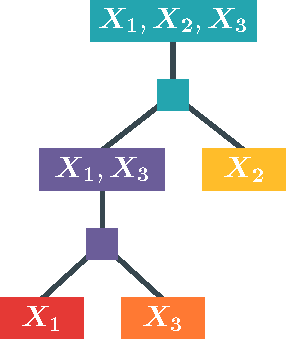
\includegraphics[width=0.8\textwidth, page=1]{assets/images/region_graphs.pdf}
%     \end{figure}
% \end{columns}
% \end{frame}

\begin{frame}[fragile]{TabPC}

    % We call \textbf{TabPC} (Tabular Data Probabilistic Circuit) the overparameterized PC we use for tabular data generation, characterized by the following design choices:

    We build probabilistic circuits for tabular data (\textbf{TabPC}) following these design choices:
    \begin{itemize}
        \item Gaussian input layers for numeric variables, categorical input layers for categorical variables.
        \item CP-layer sum-product units
        \item Structure learned with the Chow-Liu algorithm. It mixes together highly dependent variables earlier in the circuit.
        \item Preprocessing for tabular data generation (quantile normalization, handling inflated values...).
    \end{itemize}

    The only hyperparameter is the "size" of the circuit.
    %number of input units per variable and output size of the CP-layers that we both set to $K$.

\end{frame}

\begin{frame}[fragile]{Example}

    Example of TabPC built for the Magic dataset (12 features/columns).
    \begin{figure}
        \centering
        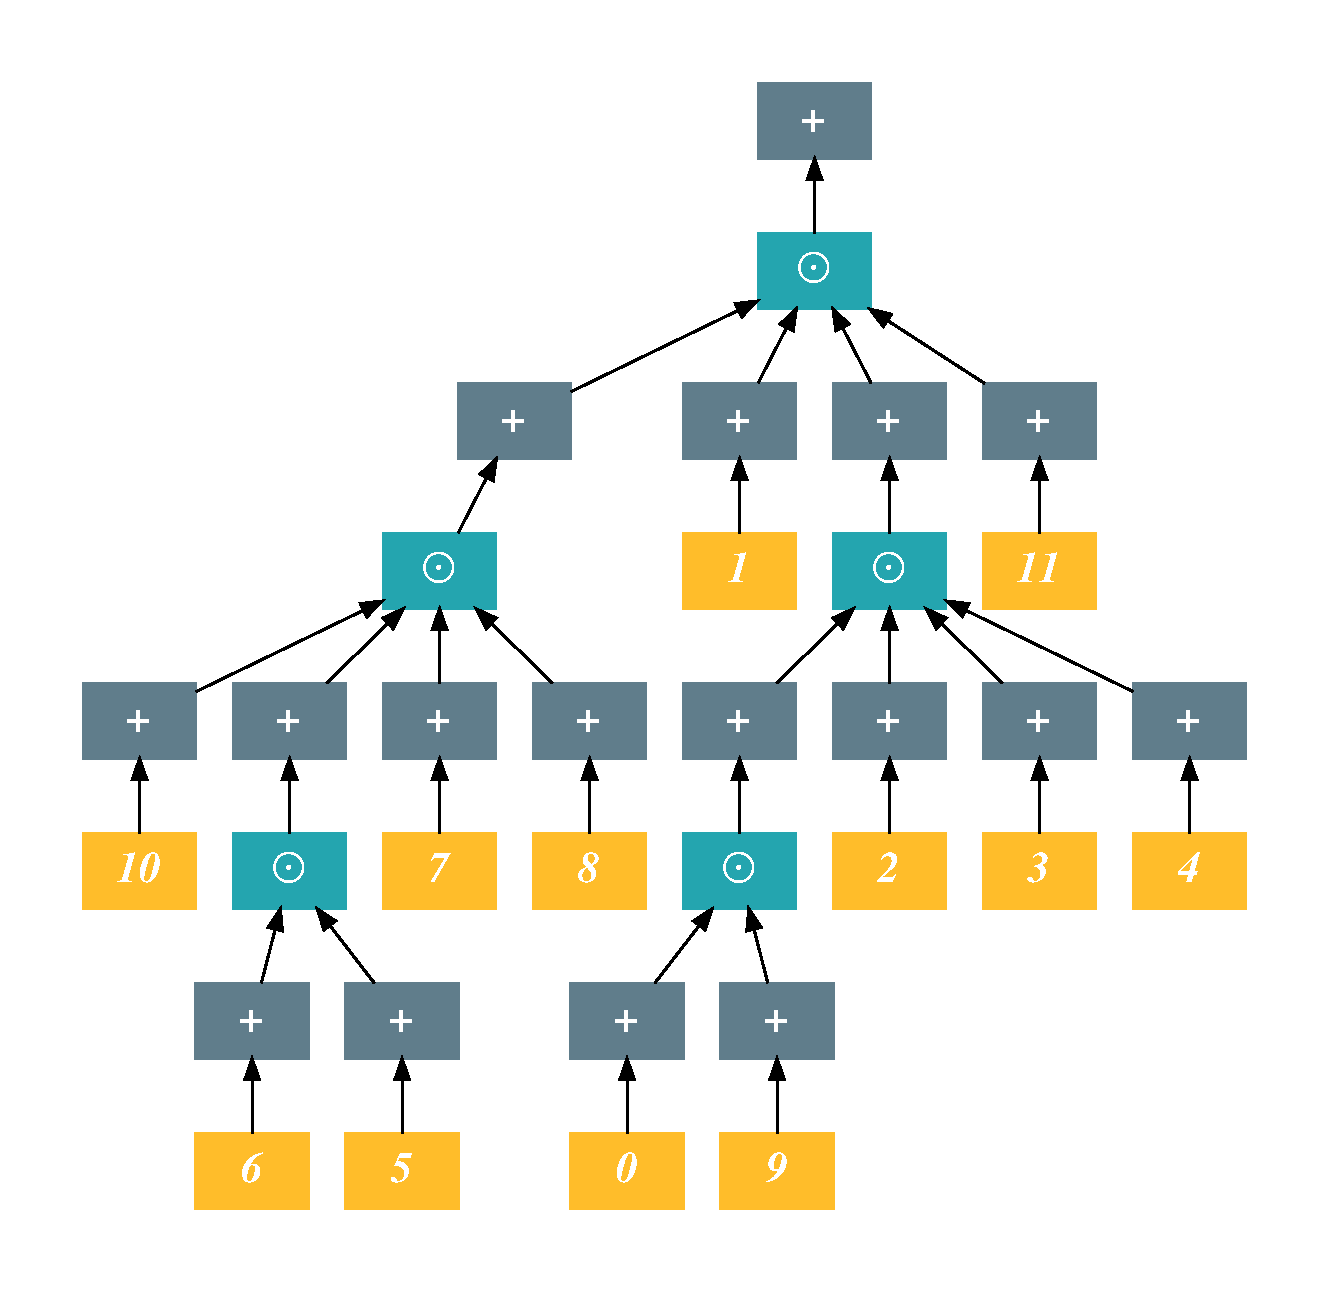
\includegraphics[width=0.5\textwidth]{assets/images/magic_graphs/circuit.pdf}
    \end{figure}

\end{frame}


\begin{frame}[fragile]{Experiments}

    We aim at comparing with state-of-the-art diffusion-based methods for tabular data generation. We run the experiments in the same settings as TabDiff \citep{tabdiff}:

    \begin{itemize}
        \item \textbf{Datasets}: 6 common datasets from the UCI machine learning repository: Adult, Beijing, Default, Diabetes, Magic, News and Shoppers.
        \item \textbf{Baselines}:
            \begin{itemize}
                \item Open-source models based on VAEs, GANs, LLMs, and diffusion.
                \item Fully Factorized model (FF) %, to understand the impact of modeling dependencies in the data.
                \item Shallow Mixture (SM) %: a mixture of fully factorized models, to assess the importance of the hierarchical structure of PCs.
            \end{itemize}
            
        \item \textbf{Metrics}:
        \begin{itemize}
            \item \textit{Fidelity} metrics: Shape (quality of marginals), Trend (quality of correlations), Detection based on logistic regression
            \item \textit{Utility} metric: Machine Learning Efficiency (MLE);
            \item \textit{Privacy} metric: Distance to Closest Record (DCR).
        \end{itemize}
    \end{itemize}

\end{frame}


\begin{frame}[fragile]{Results: Shape, Trend and LR-Detection}

    \begin{columns}
        \column{0.5\textwidth}
            \begin{figure}
                \centering
                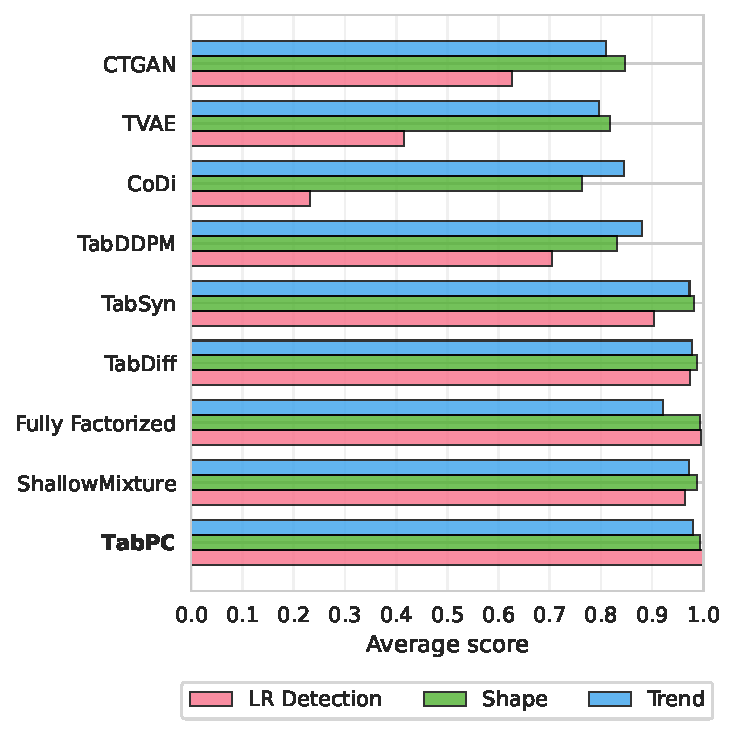
\includegraphics[width=0.95\textwidth]{images/saturation_overview.pdf}
            \end{figure}

        \column{0.5\textwidth}
            We evaluate Shape, Trend and LR-Detection metrics and report the average over the 6 datasets. All these metrics have values between 0 and 1, where 1 is the best possible score.

            \begin{itemize}
                \item Several models saturate these metrics.
                \item With proper preprocessing, even a fully factorized model can achieve good performance on these metrics.
            \end{itemize}

    \end{columns}



\end{frame}

% \begin{frame}[fragile]{Results: MLE}

%     Machine Learning Efficiency (MLE) is low for the fully factorized model, but there is also some saturation effect.
%     \begin{figure}
%         \centering
%         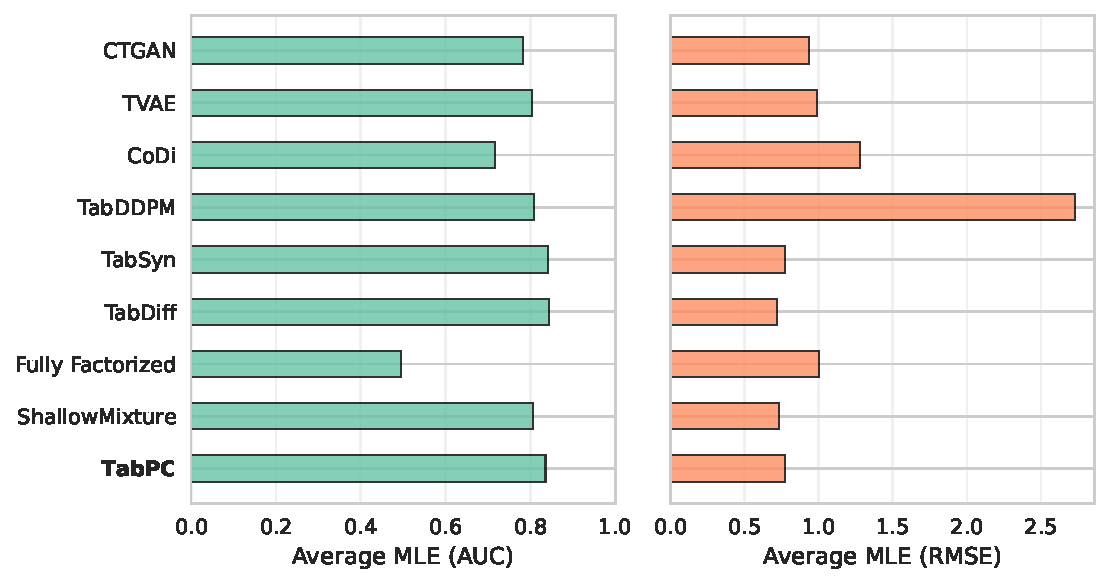
\includegraphics[width=0.8\textwidth]{images/mle.pdf}
%     \end{figure}

% \end{frame}

\begin{frame}[fragile]{Issues with Trend and LR-Detection}

    \textbf{LR-Detection}
    \begin{itemize}
        \item Logistic Regression is too easy to fool.
        \item We prove that a synthetic dataset able to replicate the mean of each feature is enough to achieve a perfect score.
        \item We suggest using a more powerful classifier or an ensemble of classifiers to make the detection more robust, as done in other works.
        We propose using XGBoost, which is powerful and fast to evaluate.
    \end{itemize}

    \textbf{Trend}
    \begin{itemize}
        \item Trend should measure the similarity of correlations, but it is heavily influenced by the quality of marginals.
        \item We propose wNMIE (weighted Normalized Mutual Information Error) which is independent of the quality of the marginals.% and only measures the quality of the correlations.
    \end{itemize}

\end{frame}

% \begin{frame}[fragile]{XGBoost-Detection}

%     \begin{columns}
%         \column{0.5\textwidth}
%             \begin{figure}
%                 \centering
%                 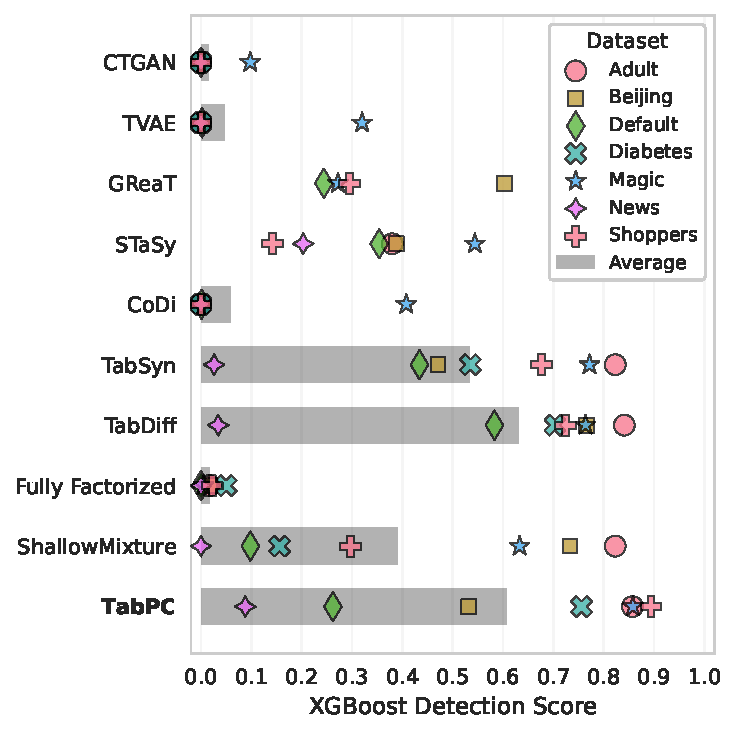
\includegraphics[width=1.0\textwidth]{images/xgb.pdf}
%             \end{figure}
%         \column{0.5\textwidth}
%             \begin{itemize}
%                 \item XGBoost better distinguishes between models.
%                 %\item wNMIWE is not influenced by marginals, fully factorized models perform poorly as expected.
%                 \item TabPC is competitive with state-of-the-art diffusion-based models.
%                 \item TabPC still struggles for some datasets, probably due to the large number of features and high correlations.
%             \end{itemize}

%     \end{columns}


% \end{frame}

% \begin{frame}[fragile]{wNMIE}

%     \begin{columns}
%         \column{0.5\textwidth}
%             \begin{figure}
%                 \centering
%                 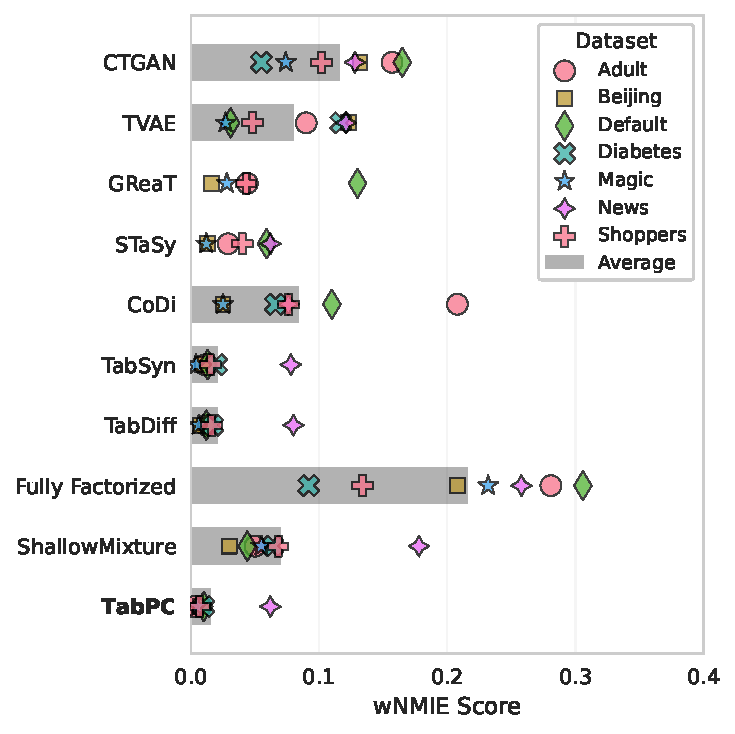
\includegraphics[width=1.00\textwidth]{images/nmi.pdf}
%             \end{figure}

%         \column{0.5\textwidth}
            
%             \begin{itemize}
%                 \item wNMIWE is not influenced by marginals, fully factorized models perform poorly as expected.
%                 \item TabPC is competitive with state-of-the-art diffusion-based models.
%             \end{itemize}

%     \end{columns}

% \end{frame}

\begin{frame}[fragile]{TabPC: Quality and Efficiency}

    \begin{columns}
        \column{0.5\textwidth}
        \begin{figure}
            \centering
            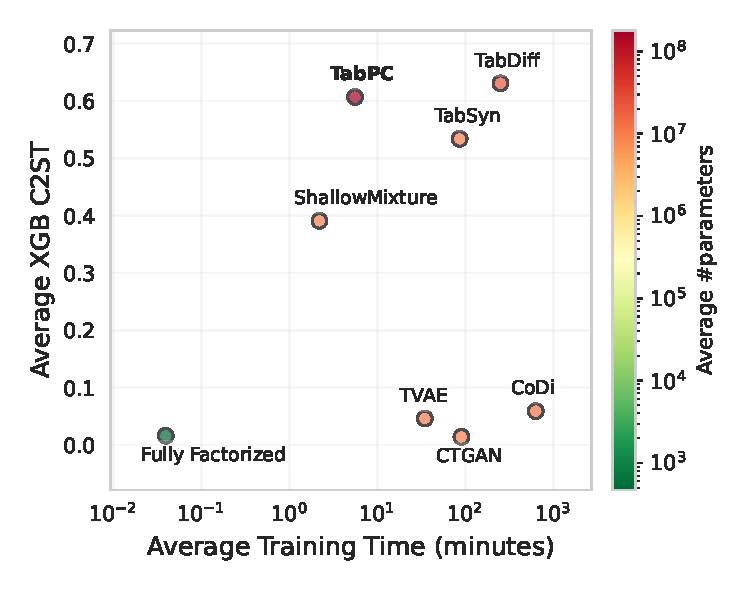
\includegraphics[width=1.0\textwidth]{images/tabpc_overview.pdf}
        \end{figure}

        \column{0.5\textwidth}
        \begin{itemize}
            \item \textbf{Quality}: TabPC is competitive with state-of-the-art diffusion-based models.
            \item \textbf{Training time}: TabPC is significantly faster to train: $\approx 40-50 \times$ faster than TabDiff.
            \item \textbf{Sampling time}: TabPC is also faster to sample from, $\approx 10 \times$ faster than TabDiff.
            \item \textbf{Number of parameters}: TabPC requires more parameters, $\approx 10 \times$ more than TabDiff.
            %\item TabPC quality of generated data is close to TabDiff.
        \end{itemize}

    \end{columns}

\end{frame}


\begin{frame}[fragile]{Discussion}

    \begin{itemize}
        \item TabPC is competitive with state-of-the-art tabular data generation models from the point of view of quality of generated data (fidelity and utility).
        \item TabPC is faster to train and sample from.
        \item TabPC is tractable, allowing the \textbf{exact} computation of probabilistic queries that are not possible with other models:
        \begin{itemize}
            \item Density evaluation
            \item Marginalization (useful for handling missing data)
            \item Conditional sampling
        \end{itemize} 
    \end{itemize}

\end{frame}

\begin{frame}[fragile]{Discussion}

    \textbf{Limitations}:
    \begin{itemize}
        \item TabPC struggles when the number of features is large and there are high correlations between them.
        \item TabPC requires more parameters.
        %\item Limited selection of datasets
    \end{itemize}

    \textbf{Future work}:
    \begin{itemize}
        \item Multivariate Gaussians as input units
        \item Variants of PCs: Probabilistic Integral Circuits \citep{gala2024probabilistic},  Sum-of-Squares Circuits \citep{loconte2025sum}, ...
        \item Expectation Maximization
        %\item Move beyond Chow-Liu trees toward more general directed acyclic graphs (DAGs).
    \end{itemize}

\end{frame}